\subsection{introduction}
	\begin{frame}{source coding}{introduction 1/3}
		\begin{itemize}
			\item	typical audio \textbf{bit rates}
				\begin{eqnarray}
					\unit[16]{bit}\cdot\unit[44100]{sps}\cdot\unit[2]{chan} &=& \unit[1411.2]{kbps}\nonumber\\
					\unit[24]{bit}\cdot\unit[192000]{sps}\cdot\unit[5]{chan} &=& \unit[23040]{kbps}\nonumber
				\end{eqnarray}
			\pause
			\vspace{-3mm}
			\item	\textbf{reasons} for bit rate reduction
				\begin{itemize}
					\item	economical reasons: cheaper transmission/storage
					\item	technical reasons: restricted storage/transmission bandwidth
				\end{itemize}
			\pause
			\item	\textbf{applications} for source coding
				\begin{itemize}
					\item	Internet: streaming, distribution, peer-2-peer, VoIP, \ldots
					\item	Media: DVD-V/A, \ldots
					\item	Portable Devices: MP3-Player, cell phones, Mini-Disc, \ldots
					\item	Broadcasting: (Digital) Radio, TV, \ldots
					\item	Cinema: DD, DTS, SDDS
					\item	\ldots
				\end{itemize}
		\end{itemize}
	\end{frame}
	\begin{frame}{source coding}{introduction 2/3}
        \setbeamercovered{invisible}
		\vspace{-12mm}
		\begin{columns}
			\column{5cm}
			How can the bitrate be reduced?
			
			\column{4cm}
			%\hspace{5mm}
			\begin{flushright}
				 
\includegraphics[scale=.08]{Graph/question-mark}
			\end{flushright}
		\end{columns}
		\pause
		\begin{enumerate}
			\item	\textbf{lossless}:\\ remove \textit{redundant} information (unnecessary to reconstruct the signal)
				\begin{itemize}
					\item	entropy coding
					\item	(linear predictive coding)
				\end{itemize}
			\pause
            \bigskip
			\item	\textbf{lossy}:\\ remove \textit{irrelevant} information (not ``missed'' by the recipient)
				\begin{itemize}
					\item	waveform coding
					\item	perceptual coding
				\end{itemize}
		\end{enumerate}
        \setbeamercovered{transparent}
	\end{frame}
	\begin{frame}{source coding}{introduction 3/3}
			\begin{figure}
				\centering
                \begin{picture}(50,50)
                    \put(0,25){\vector(1,0){50}}
                    \put(45,27){\footnotesize{\shortstack[c]{redundant}}}
                    
                    \put(25,0){\vector(0,1){50}}
                    \put(21,51){\footnotesize{\shortstack[c]{irrelevant}}}
                    
                    \put(0,0){\grid(25,25)(1.25,1.25)}
                    \put(5,10){\colorbox{white}{\framebox(15,8){\footnotesize{\shortstack[c]{\color{gtgold}{of interest}}}}}}
                 \end{picture}
					%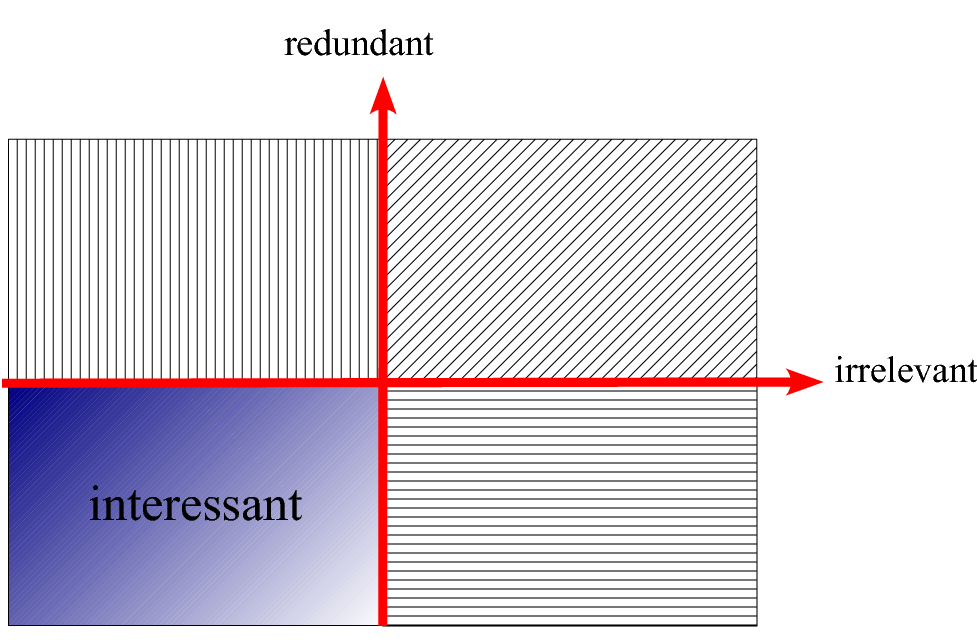
\includegraphics[scale=.3]{graph/redundancy_irrelevancy}
			\end{figure}
	\end{frame}
\subsection{information theory}
	\begin{frame}{source coding}{fundamentals: definitions}
		note: words to be transmitted are referred to as \textit{symbols}
		\pause
		\begin{block}{\textbf{information content}}
			\centering
			The less frequent a symbol, the higher its\\ \textit{information content}, \textit{self-information}, \textit{surprisal}.
			\begin{equation*}
				I_n = \log_2\left(\frac{1}{p_n} \right)
			\end{equation*}
		\end{block}
		\pause
		\begin{block}{\textbf{entropy}}
			\centering
			The entropy is the \textit{Expected Value} of the information content. It is the \textit{theoretic minimum of bits} required for transmission.
			\begin{equation*}
				H = \sum\limits_{n=0}^{N-1}{p_n\cdot I_n}
			\end{equation*}
		\end{block}
	\end{frame}

	\begin{frame}{source coding}{fundamentals: information content and entropy examples}
        \setbeamercovered{invisible}
		\begin{itemize}
			\item	\textbf{dice}: $p_n = \frac{1}{6}$
			\begin{eqnarray*}
				I_n &=& \log_2\left(\frac{1}{p_n}\right)  = 2.58\; bit\\
				H &=& 2.58\; bit % \unit[2.58]{bit}
			\end{eqnarray*}
			\pause
			\item	\textbf{imperfect dice}: $p_0 = \frac{1}{2},\; p_{1\ldots 5} = \frac{1}{10}$
			\pause
			\begin{eqnarray*}
				I_1 &=  \log_2\left(2\right)  &= 1\; bit \\
				I_{2\ldots 6} &= \log_2\left(10\right)  &= 3.32\; bit \\
				H &= \frac{1}{2}\cdot 1 + \frac{5}{10}\cdot 3.32 &= 2.16\; bit %\unit[2.16]{bit}
			\end{eqnarray*}
		\end{itemize}
        \setbeamercovered{transparent}
	\end{frame}

\subsection{entropy coding}
	\begin{frame}{source coding}{entropy coding: example 1}
		\textbf{idea: use shorter words for frequent symbols}
		\pause
		\begin{itemize}
			\item	3 possible symbols
			\begin{table}
				\begin{center}
				\begin{footnotesize}
					\begin{tabular}{lccc}
					\hline
						\textbf{symbol}  & \textbf{probability} & \textbf{word}\\
					\hline
					A & $p=0.5$	& \only<3->{$0$}\\
					B & $p=0.25$	& \only<3->{$10$}\\
					C & $p=0.25$	& \only<3->{$11$}\\
					\end{tabular}  
				\end{footnotesize}
				\end{center}
			\end{table}
			\pause
			\item	entropy
			\begin{equation*}
				H = \sum\limits_{n=0}^{N-1}{p_n\log_2\left(\frac{1}{p_n} \right)} = 1.5
			\end{equation*}
			\pause
			\item	transmit the following group of symbols: $ABCA\rightarrow \; 010110$
			
			\pause
			\item required bits:
			\begin{equation*}
				\frac{transmitted \; bits}{transmitted\; symbols} = \frac{6}{4} = 1.5
			\end{equation*}
			\pause
			$\Rightarrow$ \color{gtgold}{optimal transmission}
		\end{itemize}
	\end{frame}

	\begin{frame}{source coding}{entropy coding: example 2}
		\begin{itemize}
		
			\item 3 possible symbols
			\begin{table}
				\begin{center}
				\begin{footnotesize}
					\begin{tabular}{lccc}
					\hline
						\textbf{symbol} & \textbf{probability} & \textbf{word} \\
					\hline
					A &	 $p=0.7$	& \only<2->{$0$}\\
					B &	$p=0.2$	& \only<2->{$10$}\\
					C &	$p=0.1$	& \only<2->{$11$}\\
					\end{tabular}  
				\end{footnotesize}
				\end{center}
			\end{table}
			\pause
			\item	entropy
			\begin{equation*}
				H = \sum\limits_{n=0}^N{p_n\log_2\left(\frac{1}{p_n} \right)} = 1.11
			\end{equation*}
			\pause
			\item	transmit the following group of symbols: $ABCA\rightarrow \; 010110$

			\pause
			\item required bits:
			\begin{equation*}
				\frac{transmitted \; bits}{transmitted\; symbols} = \frac{6}{4} = 1.5
			\end{equation*}
			\pause
			$\Rightarrow$ \color{gtgold}{\textit{non}-optimal transmission}
		\end{itemize}
	\end{frame}
	
	\begin{frame}{source coding}{huffman coding: tree construction 1/2}
			\begin{table}
				\begin{center}
				\begin{footnotesize}
					\begin{tabular}{lc}
						\parbox{50mm}{sort symbols acc.\ to frequency} & 
						\begin{tabular}{cc}
							frequency & symbol\\
							5	& 1\\
							7	& 2\\
							10	& 3\\
							15	& 4\\
							20	& 5\\
							45	& 6
						\end{tabular}\\

						\parbox{50mm}{combine two lowest symbols into new entry (sum)} & 
						\begin{picture}(15,12)
							\put(6, 8){\text{12:*}}
							\put(0, 0){\text{5:1}}
							\put(13, 0){\text{7:2}}
							\put(14, 4){\line(-1,1){3}}
							\put(2, 4){\line(1,1){3}}
						\end{picture}\\
						\parbox{50mm}{add new entry to list} & 
						\begin{tabular}{cc}
							frequency & symbol\\
							10	& 3\\
							12	& *\\
							15	& 4\\
							20	& 5\\
							45	& 6
						\end{tabular}\\
						\parbox{50mm}{repeat until only one element left in the list} & 
					\end{tabular}  
				\end{footnotesize}
				\end{center}
			\end{table}
	\end{frame}
	\begin{frame}{source coding}{huffman coding: tree construction 2/2}
	\begin{center}
	\begin{picture}(70, 50)
		\only<1-2>{
			\put(0, 47){\only<2>{\textcolor{gtgold}}{\text{5:1}}}
			\put(13, 47){\only<2>{\textcolor{gtgold}}{\text{7:2}}}
			\put(26, 47){\text{10:3}}
			\put(39, 47){\text{15:4}}
			\put(52, 47){\text{20:5}}
			\put(65, 47){\text{45:6}}
		}
		\only<3-4>{
			\put(13, 47){\only<4>{\textcolor{gtgold}}{\text{10:3}}}
			\put(26, 47){\only<4>{\textcolor{gtgold}}{\text{12:*}}}
			\put(39, 47){\text{15:4}}
			\put(52, 47){\text{20:5}}
			\put(65, 47){\text{45:6}}
			
				\put(20, 39){\text{5:1}}
				\put(33, 39){\text{7:2}}
				\put(23, 43){\line(1,1){3}}
				\put(34, 43){\line(-1,1){3}}
			
		}
		\only<5-6>{
			\put(13, 47){\only<6>{\textcolor{gtgold}}{\text{15:4}}}
			\put(26, 47){\only<6>{\textcolor{gtgold}}{\text{20:5}}}
			\put(39, 47){\text{22:*}}
			\put(65, 47){\text{45:6}}
			
				\put(33, 39){\text{10:3}}
				\put(46, 39){\text{12:*}}
				\put(36, 43){\line(1,1){3}}
				\put(47, 43){\line(-1,1){3}}

					\put(40, 31){\text{5:1}}
					\put(53, 31){\text{7:2}}
					\put(43, 35){\line(1,1){3}}
					\put(54, 35){\line(-1,1){3}}
			
		}
		\only<7-8>{
			\put(26, 47){\only<8>{\textcolor{gtgold}}{\text{22:*}}}
			\put(52, 47){\only<8>{\textcolor{gtgold}}{\text{35:*}}}
			\put(65, 47){\text{45:6}}

				\put(20, 39){\text{10:3}}
				\put(33, 39){\text{12:*}}
				\put(23, 43){\line(1,1){3}}
				\put(34, 43){\line(-1,1){3}}
			
				\put(46, 39){\text{15:4}}
				\put(59, 39){\text{20:5}}
				\put(49, 43){\line(1,1){3}}
				\put(60, 43){\line(-1,1){3}}

					\put(27, 31){\text{5:1}}
					\put(40, 31){\text{7:2}}
					\put(30, 35){\line(1,1){3}}
					\put(41, 35){\line(-1,1){3}}
			
		}
		\only<9-10>{
			\put(13, 47){\only<10>{\textcolor{gtgold}}{\text{45:6}}}
			\put(39, 47){\only<10>{\textcolor{gtgold}}{\text{57:*}}}

				\put(26, 39){\text{22:*}}
				\put(52, 39){\text{35:*}}
				\put(29, 43){\line(1,1){3}}
				\put(53, 43){\line(-1,1){3}}

					\put(20, 31){\text{10:3}}
					\put(33, 31){\text{12:*}}
					\put(23, 35){\line(1,1){3}}
					\put(34, 35){\line(-1,1){3}}
				
					\put(46, 31){\text{15:4}}
					\put(59, 31){\text{20:5}}
					\put(49, 35){\line(1,1){3}}
					\put(60, 35){\line(-1,1){3}}
	
						\put(27, 23){\text{5:1}}
						\put(40, 23){\text{7:2}}
						\put(30, 27){\line(1,1){3}}
						\put(41, 27){\line(-1,1){3}}
		}
		\only<11->{
			\put(26, 47){\text{102:*}}

				\put(13, 39){\text{45:6}}
				\put(39, 39){\text{57:*}}
				\put(16, 43){\line(1,1){3}}
				\put(40, 43){\line(-1,1){3}}
	
					\put(26, 31){\text{22:*}}
					\put(52, 31){\text{35:*}}
					\put(29, 35){\line(1,1){3}}
					\put(53, 35){\line(-1,1){3}}
	
						\put(20, 23){\text{10:3}}
						\put(33, 23){\text{12:*}}
						\put(23, 27){\line(1,1){3}}
						\put(34, 27){\line(-1,1){3}}
					
						\put(46, 23){\text{15:4}}
						\put(59, 23){\text{20:5}}
						\put(49, 27){\line(1,1){3}}
						\put(60, 27){\line(-1,1){3}}
		
							\put(27, 15){\text{5:1}}
							\put(40, 15){\text{7:2}}
							\put(30, 19){\line(1,1){3}}
							\put(41, 19){\line(-1,1){3}}
		}
		\only<12->{
			\put(14, 44){\textcolor{gtgold}{\text{\textbf{0}}}}
			\put(27, 36){\textcolor{gtgold}{\text{\textbf{0}}}}
			\put(21, 28){\textcolor{gtgold}{\text{\textbf{0}}}}
			\put(47, 28){\textcolor{gtgold}{\text{\textbf{0}}}}
			\put(28, 20){\textcolor{gtgold}{\text{\textbf{0}}}}

			\put(41, 44){\textcolor{gtgold}{\text{\textbf{1}}}}
			\put(53, 36){\textcolor{gtgold}{\text{\textbf{1}}}}
			\put(34, 28){\textcolor{gtgold}{\text{\textbf{1}}}}
			\put(60, 28){\textcolor{gtgold}{\text{\textbf{1}}}}
			\put(41, 20){\textcolor{gtgold}{\text{\textbf{1}}}}
		}
	\end{picture}	
		\only<13->{
			\vspace{-18mm}
			\begin{table}
				\begin{center}
					\begin{footnotesize}
						\begin{tabular}{ccc}
							\textbf{frequency} & \textbf{symbol} & \textbf{code}\\
							5	& 1 & 1010\\
							7	& 2 & 1011\\
							10	& 3 & 100\\
							15	& 4 & 110\\
							20	& 5 & 111\\
							45	& 6 & 0
						\end{tabular}
					\end{footnotesize}
				\end{center}
			\end{table}
			%\vspace{2mm}
			\begin{itemize}
				\item[note]	no code is prefix of another code!
			\end{itemize}
		}
	\end{center}
	\end{frame}
	
	\begin{frame}{source coding}{huffman coding for audio signals}
		\begin{itemize}
			\item	Symbole: $2^w$
			\pause
			\item	PDF indicates probability per symbol
				\begin{figure}
					\centering
						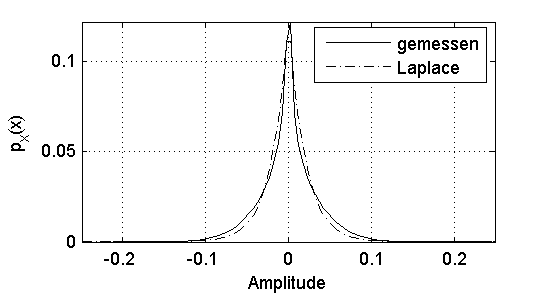
\includegraphics[scale=1.]{graph/Lerch14-9}
				\end{figure}
		\end{itemize}
	\end{frame}
	
	\begin{frame}{source coding}{arithmetic coding}
		\begin{itemize}
			\item	\textbf{Huffman coding is only optimal if $p_n = \frac{1}{2^k}$}
			\pause
            \bigskip
			\item	alternative: \textbf{arithmetic coding} 
                \begin{itemize}
                    \item   allows other probability distributions
                    \item   encodes the whole sequence in one fractional number $0.0 \leq f < 1.0$
                    \pause
                    \bigskip
                    \item   \textbf{principle}: 
                        \begin{enumerate}
                            \item   assume initial interval of $[0,1[$ 
                            \pause
                            \item   assign interval segments to all symbols, e.g. $A = [0,0.7[, B= [0.7,0.9[, C=[0.9,1[$
                            \pause
                            \item   select interval based on current symbol
                            \pause
                            \item	go to Step 2. or terminate
                        \end{enumerate}
                \end{itemize}
				%\begin{enumerate}
					%\item	set the initial interval to $[0,1[$
					%\item	split the interval into regions corresponding to probabilities, e.g. $A = [0,0.7], B= [0.7,0.9[, C=[0.9,1[$
					%\item	choose the new interval to be that of the current symbol
					%\item	go to Step 2.
					%\item	terminate with special symbol
				%\end{enumerate}	
		\end{itemize}
	\end{frame}
	
	\begin{frame}{source coding}{arithmetic coding: example}
		%\begin{itemize}
			%\item	
            \vspace{-3mm}
            sequence $ABCA$, $p_\mathrm{A} = 0.6, p_\mathrm{B}= 0.2, p_\mathrm{C}=0.1, p_\mathrm{T}=0.1$, \mbox{\footnotesize $A = [0,0.6[, B= [0.6,0.8[, C=[0.8,0.9[, T=[0.9,1[$}
            \pause
				\begin{itemize}
					\item	\textbf{decoding} 0.463: 
                        \begin{enumerate}
							\item	$0.463 \in$ segment 1 ($\rightarrow A$), set interval to $[0,0.6[$ $ \rightarrow$ {boundaries: } {\footnotesize $0,0.36,0.48,0.54,0.6$}
							\pause
                            \item	$0.463 \in$ segment 2 ($\rightarrow B$), set interval to $[0.36,0.48[$ $ \rightarrow$ {boundaries: } {\footnotesize $0.36,0.432,0.456,0.468,0.48$}
							\pause
                            \item	$0.463 \in$ segment 3 ($\rightarrow C$), set interval to $[0.456,0.468[$ $ \rightarrow$ {boundaries: } {\footnotesize $0.456,0.4632,0.4656,0.4668,0.468$}
							\pause
                            \item	$0.463 \in$ segment 1 ($\rightarrow A$), set interval to $[0.456, 0.4632[$ $ \rightarrow$ {boundaries: } {\footnotesize $0.456,0.46032,0.46176,0.46248,0.4632$}
							\pause
                            \item   $0.463 \in$ segment 4 ($\rightarrow$ terminate)
						\end{enumerate}
					\pause
					\item \textbf{encoding} 
						\begin{enumerate}
							\item	select segment 1, set interval to $[0,0.6[$
							\pause
							\item	select segment 2, set interval to $[0.36,0.48[$
							\pause
							\item	select segment 3, set interval to $[0.456,0.468[$
							\pause
							\item	select segment 1, set interval to $[0.456, 0.4632[$
							\pause
                            \item   select segment 4, set interval to $[0.46248, 0.4632[$
							\pause
							\item   choose value from last segment (e.g., 0.463) and transmit
						\end{enumerate}
				\end{itemize}
		%\end{itemize}
	\end{frame}
		
\subsection{linear prediction}
	\begin{frame}{source coding}{fundamentals: linear prediction}
		idea: use preceding samples to estimate/predict future samples.
		\begin{itemize}
			\item	\textbf{estimate the signal} x
				\begin{equation*}
					\hat{x}(i) = \sum\limits_{j=1}^{\mathcal{O}}{b_j\cdot x(i-j)}
				\end{equation*}
			\pause
			\item	prediction quality is measured by \textbf{power of prediction error}
				\begin{eqnarray*}
					e_{\mathrm{P}}(i)	&=& x(i)-\hat{x}(i)\\
							&=& x(i) - \sum\limits_{j=1}^{\mathcal{O}}{b_j\cdot x(i-j)}
				\end{eqnarray*}
		\end{itemize}						
	\end{frame}
	\begin{frame}{source coding}{fundamentals: linear prediction --- first order prediction 1/2}
        \begin{itemize}
            \item   \textbf{prediction}
                $\hat{x}(i) = b_1\cdot x(i-1)$
            \pause
            \item   \textbf{prediction error}
				\begin{eqnarray*}
                    \sigma_e^2 &=& \mathcal{E}\left\lbrace (x(i)-b_1x(i-1))^2\right\rbrace\\
                    &=& \sigma_x^2 + b_1^2 \sigma_x^2 -2b_1 r_{xx}(1)\\
                    &=& \left(1 + b_1^2 - 2b_1\rho_{xx}(1)\right) \sigma_x^2
				\end{eqnarray*}
            \pause
            \item   \textbf{optimum coefficient}: $\frac{\partial\sigma_e^2}{\partial b_1} = 0$
				\begin{eqnarray*}
                    2b_1\sigma_x^2 - 2\rho_{xx}(1)\sigma_x^2 &=& 0\\
                    b_1 &=& \rho_{xx}(1)
				\end{eqnarray*}
            \pause
            \item   \textbf{minimum prediction error power}
				\begin{eqnarray*}
                    \sigma_e^2 &=& \left(1 + b_1^2 - 2b_1\rho_{xx}(1)\right) \sigma_x^2\\
                    &=& \left(1 + \rho_{xx}(1)^2 - 2\rho_{xx}(1)\rho_{xx}(1)\right) \sigma_x^2\\
                    &=& (1-\rho_{xx}(1))\sigma_x^2
				\end{eqnarray*}
        \end{itemize}
	\end{frame}
	\begin{frame}{source coding}{fundamentals: linear prediction --- first order prediction 2/2}
        \begin{equation*}
            \sigma_e^2 = (1-\rho_{xx}(1))\sigma_x^2
        \end{equation*}
        
        \begin{itemize}
            \item             \textbf{observations}:
            \begin{itemize}
                \item   power of prediction error always smaller or equal the power of the signal
                \item   question: when is it equal to the signal?
            \end{itemize}
            \pause
            \item   \textbf{special case}: $b_1 = 1$
                \begin{eqnarray*}
                    \hat{x}(i) &=& x(i-1)\\
                    e_\mathrm{P} &=& x(i) - x(i-1)\\
                    \sigma_e^2 &=& (1 + b_1^2 -2b_1\rho_{xx}(1))\sigma_x^2\\
                    &=& 2(1-rho_{xx}(1))\sigma_x^2
                \end{eqnarray*}
        \end{itemize}
	\end{frame}
	\begin{frame}{source coding}{fundamentals: linear prediction --- prediction coefficients}
		\begin{itemize}
			\item	prediction gain depends on
				\begin{itemize}
					\item	predictor coefficients $b_j$
					\item	signal
				\end{itemize}
			\pause
			\item	optimal coefficients can be derived by finding minimum of prediction error
				\begin{equation*}
					\frac{\partial \sigma_e^2}{\partial b_j} = 0
				\end{equation*}
				$\Rightarrow$ (without derivation)
			\begin{equation*}
				r_{xx}(\eta) = \sum\limits_{j=1}^{\mathcal{O}}{b_{j,\mathrm{opt}}\cdot r_{xx}(\eta-j)} ,\;\;\;\;\; 1 \leq\eta\leq\mathcal{O} 
			\end{equation*}	
            \begin{eqnarray*}
                \vec{r}_{xx} &=& \mat{R}_{xx}\cdot \vec{b}_\mathrm{opt}\\
                \vec{b}_\mathrm{opt} &=& \mat{R}_{xx}^{-1}\cdot \vec{r}_{xx}
            \end{eqnarray*}
		\end{itemize}						
	\end{frame}
	\begin{frame}{source coding}{fundamentals: linear prediction --- summary}
		\begin{itemize}
			\item 	\textbf{predictor length}
				\begin{itemize}
					\item	rule of thumb: the longer the predictor, the better the prediction
					\item	can range from 10 coefficients to hundreds
				\end{itemize}
			\pause
            \bigskip
			\item	\textbf{predictor coefficient updates}
				\begin{itemize}
					\item	better signal adaptation if coefficients are updated block-by-block
				\end{itemize}
			\pause
            \bigskip
			\item	\textbf{input signals}
				\begin{itemize}
					\item	white noise/random processes cannot be predicted
					\item	periodic signals may theoretically be perfectly predicted
				\end{itemize}
		\end{itemize}
	\end{frame}
	\begin{frame}{source coding}{fundamentals: linear prediction --- audio example}
        \begin{columns}
            \column{.7\textwidth}
			\begin{figure}
				\centering
					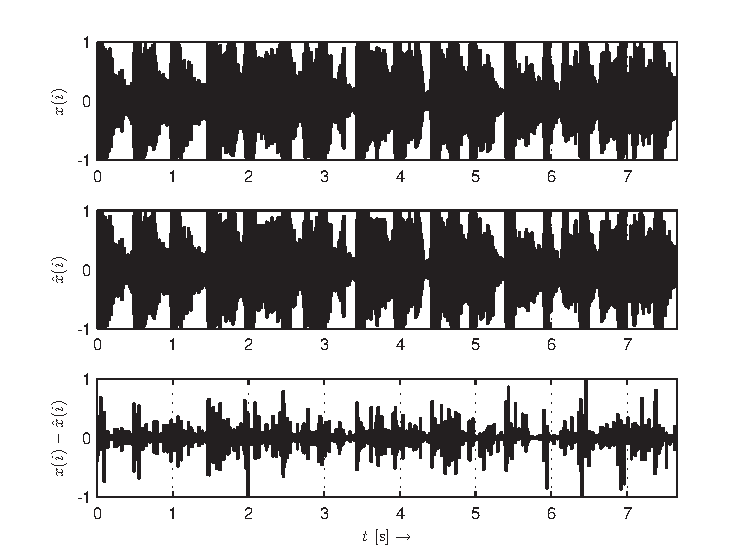
\includegraphics[scale=0.6]{\AcaGraph/linearprediction}
			\end{figure}
			\column{.3\textwidth}
                \includeaudio{audio/jamo_snippet.mp3}
                
                \bigskip
                \bigskip
                \bigskip
                order: 20 \includeaudio{audio/jamo_snippet_Pred.mp3}
                
                \bigskip
                \bigskip
                \bigskip
                \includeaudio{audio/jamo_snippet_PredError.mp3}
			\end{columns}
	\end{frame}

	\begin{frame}{source coding}{fundamentals: joint channels}
        \vspace{-5mm}
        \begin{columns}
            \column{.7\textwidth}
			\begin{figure}
				\centering
				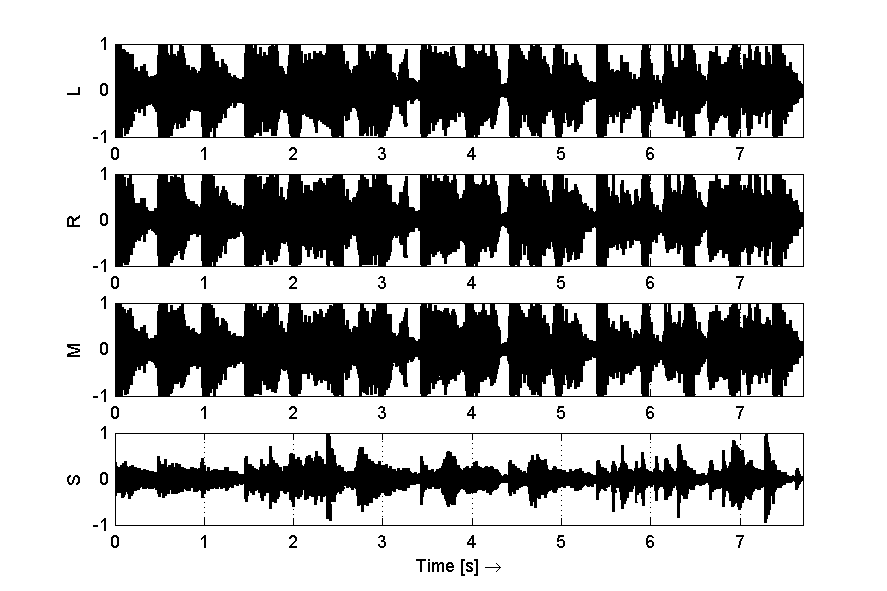
\includegraphics[scale=0.6]{Graph/ms}
			\end{figure}
			\column{.3\textwidth}
                \includeaudio{audio/jamo_snippet.mp3}
                
                \bigskip
                \bigskip
                \bigskip
                \bigskip
                \bigskip
                $M = \frac{L+R}{2}$
                \includeaudio{audio/jamo_snippet_Pred.mp3}
                
                \bigskip
                \bigskip
                $S = \frac{L-R}{2}$
                \includeaudio{audio/jamo_snippet_PredError.mp3}
			\end{columns}
			\vspace{-2mm}
            \begin{eqnarray*}
                L &=& M + S\\
                R &=& M - S 
            \end{eqnarray*}
	\end{frame}

	
